% ==============================================================================
% Section 3: Methodology (03-methodology.tex)
% ==============================================================================

\section{방법론 (Methodology)}
\label{sec:method}

\subsection{전체 시스템 개요 및 처리 흐름}
\label{sec:method:overview}

본 연구는 스마트팜 현장의 자원 제약 환경(8GB RAM)에서 근거 기반 실시간 응답을 제공하는 온디바이스 RAG 시스템을 제안한다. \cref{fig:architecture}는 시스템의 End-to-End 아키텍처를 3-Column 가로 배치로 제시한다:

\begin{itemize}
    \item \textbf{Phase 1 (좌측, 청색)}: 데이터 수집 및 인덱스 구축 (Offline, One-time)
    \item \textbf{Phase 2 (중앙, 청색)}: 런타임 추론 파이프라인 (Online, Per-query)
    \item \textbf{Evaluation Protocol (우측, 주황색)}: Dataset 생성 + 검증/평가 방법론
\end{itemize}

\subsubsection{End-to-End 처리 흐름}
\label{sec:method:overview:e2e}

% TODO: Figure 1 - See figures/fig-architecture.tex
\begin{figure}[htbp]
\centering
% % Figure 1: Main 3-Column Pipeline Architecture
% Design Spec: docs/era-smartfarm-rag/paper/figures/ARCHITECTURE_FIGURE_DESIGN.md
% TODO: Replace with actual TikZ diagram implementing full 3-column layout

\begin{figure}[htbp]
\centering
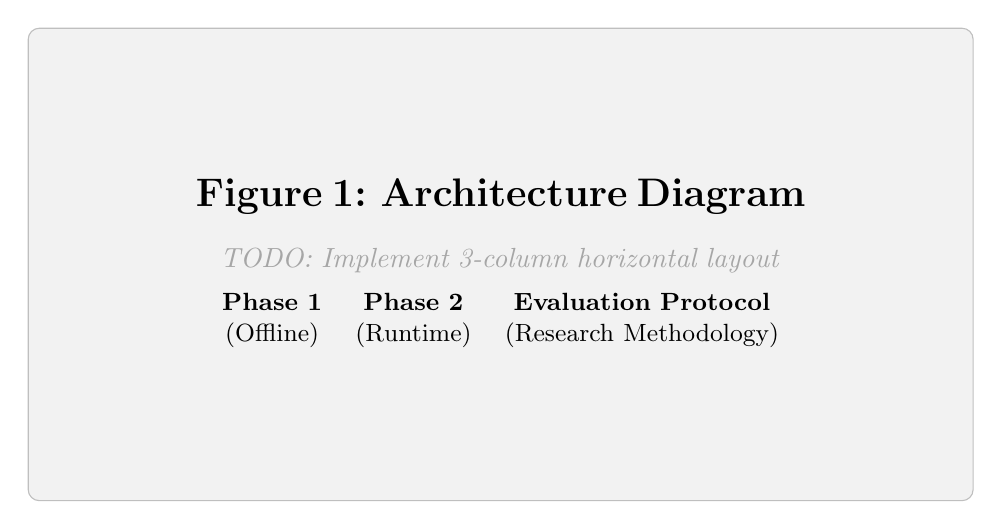
\begin{tikzpicture}
  \node[rectangle, draw=gray!50, fill=gray!10, minimum width=12cm, minimum height=6cm, rounded corners] (placeholder) {};
  \node[text width=10cm, align=center] at (placeholder.center) {
    \textbf{\Large Figure 1: Architecture Diagram}\\[1em]
    \textcolor{gray!70}{\textit{TODO: Implement 3-column horizontal layout}}\\[0.5em]
    \small
    \begin{tabular}{ccc}
    \textbf{Phase 1} & \textbf{Phase 2} & \textbf{Evaluation Protocol} \\
    (Offline) & (Runtime) & (Research Methodology) \\
    \end{tabular}
  };
\end{tikzpicture}
\caption{ERA-SmartFarm-RAG: End-to-End Research Pipeline with 3-column architecture showing Phase 1 (Data \& Index Build), Phase 2 (Runtime Inference with HybridDAT), and Evaluation Protocol (Dataset Generation + Metrics).}
\label{fig:architecture}
\end{figure}

\fbox{\parbox{0.9\textwidth}{\centering\vspace{2cm}
\textit{[Figure Placeholder: ERA-SmartFarm-RAG End-to-End Research Pipeline (3-Column Horizontal Layout)]}
\vspace{2cm}}}
\caption{ERA-SmartFarm-RAG End-to-End Research Pipeline. Phase 1 (좌측): 오프라인 데이터 수집 및 인덱스 구축. Phase 2 (중앙): 런타임 추론 파이프라인. Evaluation Protocol (우측): 데이터셋 생성 및 평가 방법론.}
\label{fig:architecture}
\end{figure}

시스템 파이프라인은 7단계로 구성되며, \cref{tab:pipeline-stages}에 각 단계의 역할을 정리하였다.

\begin{table}[htbp]
\centering
\caption{System Pipeline 7단계 구성}
\label{tab:pipeline-stages}
\begin{tabular}{@{}clp{8cm}@{}}
\toprule
\textbf{단계} & \textbf{구성요소} & \textbf{설명} \\
\midrule
1 & Data Collection & Web Crawl (Wikipedia, Britannica), 농촌진흥청 PDF, 스마트팜코리아 가이드, EN/KO Bilingual \\
2 & Preprocessing & OCR (EasyOCR), Sentence-window chunking, Metadata tagging (crop, causal, numeric), EN$\rightarrow$KO Translation \\
3 & Knowledge Store & dense.faiss (mmap), sparse.pkl (TF-IDF), Causal Graph (in-memory), ontology.json (6 types) \\
4 & Query Analysis & 온톨로지 매칭, Dynamic Alpha (수치$\rightarrow\alphasparse$+0.2, 환경/영양$\rightarrow\alphasparse$+0.1, 병해/재배$\rightarrow\alphapath$\textasciitilde0.3-0.4) \\
5 & HybridDAT Retrieval & 3채널 하이브리드 검색 (Dense FAISS + Sparse TF-IDF + PathRAG BFS 2-hop) + Score Fusion \\
6 & Context Shaping & Crop Filter (+0.5/$\times$0.15), Semantic Dedup ($\theta$=0.85), Memory-aware Reranking \\
7 & LLM Generation & Qwen3-0.6B Q4\_K\_M, Fallback Chain (Exact Cache$\rightarrow$Similar Cache$\rightarrow$Template$\rightarrow$Search-only) \\
\bottomrule
\end{tabular}
\end{table}

\textbf{Evaluation Protocol (dataset-pipeline 기반)}은 다음과 같은 방법론을 적용한다:

\begin{itemize}
    \item \textbf{Dataset Generation}: Self-Instruct (Wang et al., ACL 2023)로 Seed questions에서 다양한 질문을 자동 생성하고, Evol-Instruct (Xu et al., ICLR 2023)로 복잡도를 점진적으로 진화시킨다 (basic$\rightarrow$intermediate$\rightarrow$advanced). RAFT (Zhang et al., COLM 2024)로 Context-grounded answer generation을 수행한다.
    \item \textbf{Quality Evaluation}: LLM-as-a-Judge (Zheng et al., NeurIPS 2024)와 Prometheus (Kim et al., NeurIPS 2024)를 활용하여 Groundedness, Accuracy, Completeness 등 다차원 품질을 평가한다.
    \item \textbf{QA Dataset}: 220 pairs, 6 categories, ROUGE-L diversity 0.93, Groundedness 0.52
    \item \textbf{Evaluation Metrics}: Retrieval Quality (Recall@k, Precision@k, MRR), Edge Performance (Latency p50/p95/p99, Memory Usage, Throughput), Answer Quality (LLM-as-a-Judge Score 1-5, Hallucination Rate)
\end{itemize}

\textbf{핵심 설계 원칙}은 다음과 같다:

\begin{enumerate}
    \item \textbf{오프라인 사전 구축}: 인덱싱/인과관계 그래프(in-memory 빌드)는 1회 오프라인으로 수행하여 런타임 부하 최소화
    \item \textbf{메모리 효율}: mmap 기반 lazy loading으로 전체 인덱스를 RAM에 올리지 않음
    \item \textbf{도메인 특화}: 온톨로지 + Dynamic Alpha 휴리스틱으로 범용 RAG 대비 검색 품질 향상
    \item \textbf{데이터셋 생성}: 검증된 연구 방법론 (Self-Instruct, Evol-Instruct, RAFT, LLM-as-a-Judge) 적용
    \item \textbf{검증 분리}: Groundedness Checks + Prompt Constraints는 Evaluation Protocol로 분리하여 학술적 규약 준수
\end{enumerate}

\subsubsection{시스템 아키텍처 (6계층 스택)}
\label{sec:method:overview:architecture}

본 시스템은 스마트팜 도메인에 특화된 온디바이스 하이브리드 RAG로, 6계층 스택 아키텍처로 구성된다.

\subsubsection{리소스 제약 및 설계 목표}
\label{sec:method:overview:constraints}

엣지 환경의 리소스 제약을 명확히 정의하고, 이를 기반으로 각 컴포넌트를 설계하였다. \cref{tab:resource-constraints}에 리소스 제약 사항을 정리하였다.

\begin{table}[htbp]
\centering
\caption{리소스 제약 및 설계 목표}
\label{tab:resource-constraints}
\begin{tabular}{@{}lllp{4cm}@{}}
\toprule
\textbf{리소스 항목} & \textbf{최소 사양} & \textbf{권장 사양} & \textbf{설계 근거} \\
\midrule
RAM & 8GB & 16GB & Jetson Orin Nano 타겟 \\
저장공간 & 10GB & 20GB & GGUF 모델 + FAISS 인덱스 \\
목표 지연 & p95 < 500ms & p95 < 300ms & 실시간 현장 응답 \\
LLM 메모리 & \textasciitilde2.5GB & \textasciitilde4GB & Q4\_K\_M 양자화 기준 \\
처리량 & 3 QPS & 8 QPS & CPU 단독 환경 \\
\bottomrule
\end{tabular}
\end{table}

\subsubsection{6계층 아키텍처}
\label{sec:method:overview:layers}

% TODO: Figure 2 - See figures/fig-layer-architecture.tex
\begin{figure}[htbp]
\centering
% \input{figures/fig-layer-architecture}
\fbox{\parbox{0.9\textwidth}{\centering\vspace{2cm}
\textit{[Figure Placeholder: 6-Layer Stack Architecture]}
\vspace{2cm}}}
\caption{6-Layer Stack Architecture. L0: Device \& Runtime (llama.cpp, FAISS mmap). L1: On-device Knowledge Store. L2: Retrieval Core (HybridDAT). L3: Context Shaping. L4: Generation \& Grounding. L5: Application \& Policy.}
\label{fig:layer-architecture}
\end{figure}

\cref{tab:layer-roles}에 각 계층의 핵심 역할을 정리하였다.

\begin{table}[htbp]
\centering
\caption{6계층 아키텍처 역할}
\label{tab:layer-roles}
\begin{tabular}{@{}clp{6cm}@{}}
\toprule
\textbf{계층} & \textbf{역할} & \textbf{핵심 컴포넌트} \\
\midrule
L5 & 사용자 인터페이스 및 정책 & FastAPI, Streamlit, 폴백 정책 \\
L4 & 응답 생성 및 그라운딩 & 프롬프트 템플릿, 템플릿 응답기 \\
L3 & 컨텍스트 압축 (논문 핵심) & 작물 필터, 중복 제거, 리랭킹 \\
L2 & 3채널 하이브리드 검색 & Dense, Sparse, PathRAG 융합 \\
L1 & 온디바이스 지식 저장소 & FAISS 인덱스, 인과관계 그래프, 온톨로지 \\
L0 & 디바이스 런타임 & llama.cpp, 임베딩 모델, FAISS \\
\bottomrule
\end{tabular}
\end{table}

%------------------------------------------------------------------------------
\subsection{데이터 수집 및 전처리 파이프라인}
\label{sec:method:data}

\subsubsection{데이터 수집}
\label{sec:method:data:collection}

본 연구의 지식 베이스는 다음 세 가지 유형의 농업 문서로 구성된다 (\cref{tab:data-sources}).

\begin{table}[htbp]
\centering
\caption{데이터 수집 현황}
\label{tab:data-sources}
\begin{tabular}{@{}lllc@{}}
\toprule
\textbf{데이터 유형} & \textbf{출처} & \textbf{형식} & \textbf{수량} \\
\midrule
재배 매뉴얼 & 농촌진흥청, 도농업기술원 & PDF, 이미지 & \textasciitilde50개 \\
기술 가이드 & 스마트팜 코리아, 농업기술실용화재단 & 웹 문서, PDF & \textasciitilde30개 \\
작업 기록 & 현장 농가 메모, Q\&A 게시판 & 텍스트, 이미지 & \textasciitilde20개 \\
\bottomrule
\end{tabular}
\end{table}

\textbf{수집 기준}:
\begin{itemize}
    \item 와사비 재배에 직접 관련된 문서 우선
    \item 환경 관리(온도, 습도, EC, pH)에 대한 수치 정보 포함 문서
    \item 병해충 진단 및 해결책이 명시된 문서
\end{itemize}

\subsubsection{전처리 파이프라인}
\label{sec:method:data:preprocessing}

% TODO: Figure 3 - See figures/fig-preprocessing.tex
\begin{figure}[htbp]
\centering
% \input{figures/fig-preprocessing}
\fbox{\parbox{0.9\textwidth}{\centering\vspace{2cm}
\textit{[Figure Placeholder: Data Preprocessing Pipeline]}
\vspace{2cm}}}
\caption{Data Preprocessing Pipeline. 입력 문서(PDF, 이미지, 텍스트)에서 OCR 처리, 시맨틱 청킹, 메타데이터 추출을 거쳐 Knowledge Store로 전달한다.}
\label{fig:preprocessing}
\end{figure}

\subsubsection{OCR 및 텍스트 정규화}
\label{sec:method:data:ocr}

이미지 기반 문서(스캔 PDF, 현장 사진)는 \textbf{EasyOCR}을 사용하여 텍스트로 변환한다.

\textbf{정규화 규칙}:
\begin{itemize}
    \item 온도: ``25도'', ``25°C'', ``섭씨 25도'' $\rightarrow$ \texttt{25\textcelsius}
    \item EC: ``2.5 dS/m'', ``EC 2.5'', ``전기전도도 2.5'' $\rightarrow$ \texttt{EC 2.5 dS/m}
    \item pH: ``pH6.5'', ``산도 6.5'' $\rightarrow$ \texttt{pH 6.5}
\end{itemize}

\begin{lstlisting}[language=Python, caption={Normalization Patterns}, label={lst:normalization}, escapechar=|]
# Normalization example
NORMALIZATION_PATTERNS = {
    r'(\d+\.?\d*)\s*(C|celsius)': r'\1 C',
    r'(EC)\s*(\d+\.?\d*)': r'EC \2 dS/m',
    r'(pH)\s*(\d+\.?\d*)': r'pH \2',
}
\end{lstlisting}

\subsubsection{시맨틱 청킹 전략}
\label{sec:method:data:chunking}

단순 길이 기반 분할 대신, 문서의 \textbf{의미 구조}를 보존하는 청킹을 적용한다 (\cref{tab:chunking-strategy}).

\begin{table}[htbp]
\centering
\caption{시맨틱 청킹 전략}
\label{tab:chunking-strategy}
\begin{tabular}{@{}llc@{}}
\toprule
\textbf{전략} & \textbf{설명} & \textbf{토큰 범위} \\
\midrule
섹션 기반 & 제목/소제목으로 1차 분할 & 가변 \\
의미 병합 & 짧은 섹션은 연관 섹션과 병합 & 200--500 \\
오버랩 & 문맥 연속성을 위한 중복 구간 & 50 \\
\bottomrule
\end{tabular}
\end{table}

\textbf{청킹 파라미터}:
\begin{itemize}
    \item \texttt{CHUNK\_MIN\_TOKENS}: 200 (너무 짧은 청크 방지)
    \item \texttt{CHUNK\_MAX\_TOKENS}: 500 (컨텍스트 윈도우 효율)
    \item \texttt{CHUNK\_OVERLAP}: 50 (문맥 연속성)
\end{itemize}

\subsubsection{메타데이터 자동 추출}
\label{sec:method:data:metadata}

각 청크에 대해 다음 메타데이터를 규칙 기반으로 자동 추출한다 (\cref{tab:metadata-extraction}).

\begin{table}[htbp]
\centering
\caption{메타데이터 추출 방법}
\label{tab:metadata-extraction}
\begin{tabular}{@{}lll@{}}
\toprule
\textbf{메타데이터} & \textbf{추출 방법} & \textbf{용도} \\
\midrule
crop & 온톨로지 매칭 (작물명 사전) & 작물 필터링 \\
category & 키워드 분류기 & 도메인 분석 \\
causal\_role & 패턴 매칭 (원인/결과/해결 키워드) & PathRAG 그래프 \\
numeric\_info & 정규표현식 추출 & Sparse 검색 강화 \\
source & 원본 파일명 + 페이지 & 근거 추적 \\
\bottomrule
\end{tabular}
\end{table}

\begin{lstlisting}[language=Python, caption={Metadata Extraction Example}, label={lst:metadata}]
def extract_metadata(chunk_text: str) -> dict:
    return {
        "crop": ontology_matcher.match_crop(chunk_text),
        "category": classify_category(chunk_text),
        "causal_role": detect_causal_role(chunk_text),
        "numeric_info": extract_numeric_values(chunk_text),
        "source": {"file": source_file, "page": page_num}
    }
\end{lstlisting}

%------------------------------------------------------------------------------
\subsection{스마트팜 온톨로지}
\label{sec:method:ontology}

\subsubsection{설계 배경}
\label{sec:method:ontology:background}

온톨로지 설계는 Stanford 온톨로지 구축 방법론과 기존 농업 온톨로지 연구~\cite{bhuyan2021ontology,ahmadzai2024innovative,cornei2024ontology}를 참조하여 스마트팜 도메인에 적합한 6개 개념 유형을 정의하였다. CropDP-KG~\cite{yan2025cropdpkg}의 엔티티 구조와 AgriKG~\cite{chen2019agrikg}의 농업 엔티티 분류를 참고하여 한국 스마트팜 환경에 맞게 구성하였다.

\subsubsection{개념 유형 정의}
\label{sec:method:ontology:types}

% TODO: Figure 4 - See figures/fig-ontology.tex
\begin{figure}[htbp]
\centering
% % Figure 4: SmartFarm Domain Ontology
% TODO: Replace with actual TikZ diagram showing 6-type ontology + concept graph

\begin{figure}[htbp]
\centering
\begin{tikzpicture}
  \node[rectangle, draw=gray!50, fill=gray!10, minimum width=10cm, minimum height=5cm, rounded corners] (placeholder) {};
  \node[text width=9cm, align=center] at (placeholder.center) {
    \textbf{\Large Figure 4: SmartFarm Domain Ontology}\\[1em]
    \textcolor{gray!70}{\textit{TODO: Implement 6-type ontology diagram}}\\[0.5em]
    \small
    \begin{tabular}{cc}
    \multicolumn{2}{c}{\textbf{6 Ontology Types:}} \\
    crop (작물) & env (환경) \\
    nutrient (양액) & disease (병해) \\
    stage (생육) & practice (재배) \\
    \multicolumn{2}{c}{+ aliases per concept} \\
    \end{tabular}
  };
\end{tikzpicture}
\caption{SmartFarm domain ontology with 6 concept types (crop, environment, nutrient, disease, growth stage, practice) and their aliases for robust query matching.}
\label{fig:ontology}
\end{figure}

\fbox{\parbox{0.9\textwidth}{\centering\vspace{2cm}
\textit{[Figure Placeholder: SmartFarm Domain Ontology (6 Concept Types)]}
\vspace{2cm}}}
\caption{SmartFarm Domain Ontology. 6개 개념 유형(crop, env, nutrient, disease, stage, practice)과 각 유형별 예시 엔티티를 나타낸다.}
\label{fig:ontology}
\end{figure}

\cref{tab:ontology-types}에 6개 개념 유형의 정의와 근거를 정리하였다.

\begin{table}[htbp]
\centering
\caption{온톨로지 개념 유형 정의}
\label{tab:ontology-types}
\begin{tabular}{@{}lp{4cm}p{4cm}l@{}}
\toprule
\textbf{유형} & \textbf{설명} & \textbf{예시} & \textbf{근거} \\
\midrule
crop & 재배 작물 & 와사비, 토마토, 딸기 & CropDP-KG~\cite{yan2025cropdpkg} \\
env & 환경 요소 & 온도, 습도, EC, pH, CO$_2$ & 스마트팜 IoT 센서 데이터 표준~\cite{cornei2024ontology} \\
nutrient & 영양소 & 양액, 비료, 관수 & 농업 지식 베이스~\cite{bhuyan2021ontology} \\
disease & 병해충 & 흰가루병, 뿌리썩음병, 연부병 & CropDP-KG~\cite{yan2025cropdpkg,wang2024tomatokg} \\
stage & 생육 단계 & 육묘, 정식, 생육, 수확 & 작물 생육 모델~\cite{sitokonstantinou2024causal} \\
practice & 재배 실천 & 차광, 환기, 난방, 살균 & 농업 실천 온톨로지~\cite{bhuyan2021ontology,ahmadzai2024innovative} \\
\bottomrule
\end{tabular}
\end{table}

각 개념은 동의어/유의어 목록(alias)을 포함한다. 예를 들어 ``와사비''의 alias에는 ``산와사비'', ``본와사비''가 포함되어 사용자가 어떤 표현을 쓰더라도 동일 개념으로 인식한다.

%------------------------------------------------------------------------------
\subsection{3채널 하이브리드 검색 (HybridDAT)}
\label{sec:method:hybriddat}

\subsubsection{설계 근거}
\label{sec:method:hybriddat:rationale}

Dense retrieval은 의미적 유사성 검색에 강하지만 ``EC 2.5 dS/m'' 같은 수치 정보 매칭에 취약하다. Sparse retrieval은 정확한 키워드 매칭에 강하지만 의미적 유사성을 놓칠 수 있다~\cite{karpukhin2020dense}. 본 시스템은 Dense-Sparse-PathRAG 3채널 융합과 질의 특성에 따른 동적 가중치 조정(Dynamic Alpha Tuning)을 적용한다.

\subsubsection{HybridDATRetriever 플로우}
\label{sec:method:hybriddat:flow}

% TODO: Figure 5 - See figures/fig-hybriddat.tex
\begin{figure}[htbp]
\centering
% % Figure 5: HybridDAT Retrieval Flow
% TODO: Replace with actual TikZ diagram showing 3-channel retrieval + dynamic alpha tuning

\begin{figure}[htbp]
\centering
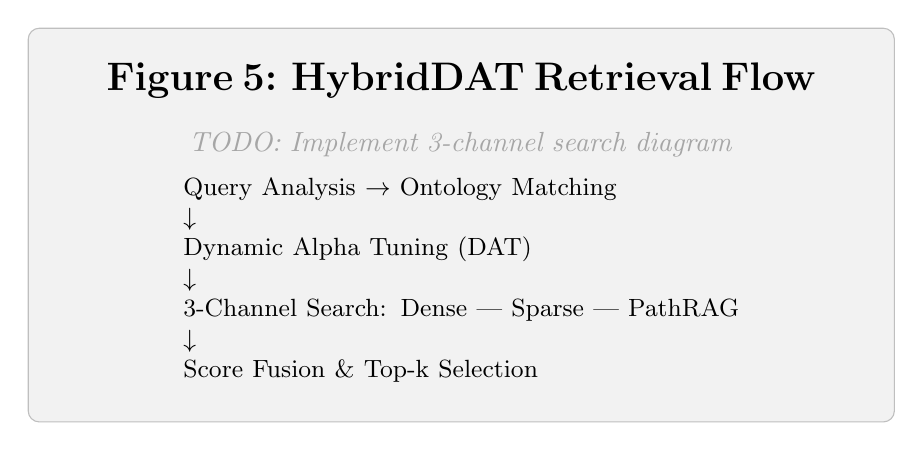
\begin{tikzpicture}
  \node[rectangle, draw=gray!50, fill=gray!10, minimum width=11cm, minimum height=5cm, rounded corners] (placeholder) {};
  \node[text width=10cm, align=center] at (placeholder.center) {
    \textbf{\Large Figure 5: HybridDAT Retrieval Flow}\\[1em]
    \textcolor{gray!70}{\textit{TODO: Implement 3-channel search diagram}}\\[0.5em]
    \small
    \begin{tabular}{l}
    Query Analysis $\rightarrow$ Ontology Matching \\
    $\downarrow$ \\
    Dynamic Alpha Tuning (DAT) \\
    $\downarrow$ \\
    3-Channel Search: Dense | Sparse | PathRAG \\
    $\downarrow$ \\
    Score Fusion \& Top-k Selection \\
    \end{tabular}
  };
\end{tikzpicture}
\caption{HybridDAT retrieval pipeline with dynamic alpha tuning based on query characteristics. The system adjusts weights between dense (FAISS), sparse (TF-IDF), and PathRAG channels according to query type (numeric/disease/practice).}
\label{fig:hybriddat}
\end{figure}

\fbox{\parbox{0.9\textwidth}{\centering\vspace{2.5cm}
\textit{[Figure Placeholder: HybridDAT Retrieval Flow (3채널 융합 검색)]}
\vspace{2.5cm}}}
\caption{HybridDAT Retrieval Flow. 질의 분석 $\rightarrow$ 온톨로지 매칭 $\rightarrow$ Dynamic Alpha 계산 $\rightarrow$ 3채널 병렬 검색 $\rightarrow$ Score Fusion.}
\label{fig:hybriddat}
\end{figure}

\subsubsection{동적 가중치 규칙 (Dynamic Alpha)}
\label{sec:method:hybriddat:alpha}

질의 내용을 분석하여 가중치를 자동 결정한다 (\cref{tab:dynamic-alpha}).

\begin{table}[htbp]
\centering
\caption{Dynamic Alpha 규칙}
\label{tab:dynamic-alpha}
\begin{tabular}{@{}lcccp{4cm}@{}}
\toprule
\textbf{질의 특성} & $\alphadense$ & $\alphasparse$ & $\alphapath$ & \textbf{설계 근거} \\
\midrule
일반 질의 & 0.5 & 0.5 & 0.0 & 의미 검색과 키워드 매칭 균형 \\
수치/단위 포함 (``EC 2.5'', ``25\textcelsius'') & 0.3 & 0.7 & 0.0 & 수치는 정확히 일치해야 함~\cite{gong2025application} \\
병해/재배 관련 (``흰가루병 원인'') & 0.35 & 0.35 & 0.3 & 인과관계 탐색 활성화 \\
\bottomrule
\end{tabular}
\end{table}

최종 스코어 융합은 다음 수식으로 계산된다:

\begin{equation}
\text{final} = \alphadense \cdot D + \alphasparse \cdot S + \alphapath \cdot P
\label{eq:score-fusion}
\end{equation}

여기서 $D$, $S$, $P$는 각각 Dense, Sparse, PathRAG 채널의 Min-Max 정규화된 스코어이다.

%------------------------------------------------------------------------------
\subsection{인과관계 그래프 (PathRAG-lite)}
\label{sec:method:pathrag}

\subsubsection{설계 배경}
\label{sec:method:pathrag:background}

농업 도메인에서 ``고수온 $\rightarrow$ 연부병 발생 $\rightarrow$ 수온 관리'' 같은 인과 체인이 핵심 정보 구조를 형성한다~\cite{sitokonstantinou2024causal}. GraphRAG~\cite{edge2024graphrag}는 LLM으로 개체와 관계를 추출하므로 구축 비용이 높다(문서 1000개당 GPT-4 \$100+). 본 시스템은 규칙 기반 패턴 매칭으로 인과관계 그래프를 구축하여 비용을 \$0으로 절감한다.

\subsubsection{인과관계 역할 분류}
\label{sec:method:pathrag:roles}

텍스트 패턴 매칭으로 문서의 역할을 분류한다 (\cref{tab:causal-roles}).

\begin{table}[htbp]
\centering
\caption{인과관계 역할 분류}
\label{tab:causal-roles}
\begin{tabular}{@{}lll@{}}
\toprule
\textbf{역할} & \textbf{판별 패턴} & \textbf{예시 문장} \\
\midrule
Cause & ``원인'', ``때문'', ``\textasciitilde하면'', ``높으면'', ``낮으면'' & ``고온 환경에서는 화분 활력이 저하된다'' \\
Effect & ``결과'', ``증상'', ``문제'', ``장애'', ``저하'' & ``착과율이 떨어지는 문제가 발생한다'' \\
Solution & ``관리'', ``해야'', ``방법'', ``조치'', ``예방'' & ``야간 온도를 18\textcelsius{} 이하로 관리해야 한다'' \\
\bottomrule
\end{tabular}
\end{table}

\subsubsection{PathRAG-lite BFS 탐색}
\label{sec:method:pathrag:bfs}

PathRAG~\cite{chen2025pathrag}의 경로 탐색 개념을 차용한 경량 구현이다. BFS(너비 우선 탐색) 기반 2-hop 탐색으로 원인$\rightarrow$결과$\rightarrow$해결책 문서를 수집한다.

% TODO: Figure 6 - See figures/fig-pathrag-bfs.tex
\begin{figure}[htbp]
\centering
% \input{figures/fig-pathrag-bfs}
\fbox{\parbox{0.9\textwidth}{\centering\vspace{2.5cm}
\textit{[Figure Placeholder: PathRAG-lite BFS 2-hop Traversal]}
\vspace{2.5cm}}}
\caption{PathRAG-lite BFS 2-hop Traversal. 질의에서 온톨로지 매칭된 개념 노드를 시작으로, causes/solved\_by 엣지를 따라 2-hop 범위의 관련 문서를 수집한다.}
\label{fig:pathrag-bfs}
\end{figure}

\subsubsection{그래프 스키마}
\label{sec:method:pathrag:schema}

CropDP-KG~\cite{yan2025cropdpkg}와 AgriKG~\cite{chen2019agrikg}의 스키마 설계를 참조하여 구성하였다.

\textbf{노드 타입}: practice(문서), crop, env, disease, nutrient, stage

\textbf{엣지 타입}은 \cref{tab:edge-types}에 정리하였다.

\begin{table}[htbp]
\centering
\caption{그래프 엣지 타입}
\label{tab:edge-types}
\begin{tabular}{@{}lll@{}}
\toprule
\textbf{타입} & \textbf{의미} & \textbf{참조} \\
\midrule
recommended\_for & 작물 $\rightarrow$ 실천 & AgriKG~\cite{chen2019agrikg} \\
associated\_with & 병해 $\rightarrow$ 실천 & CropDP-KG~\cite{yan2025cropdpkg} \\
mentions & 실천 $\rightarrow$ 개념 & 농업 온톨로지~\cite{ahmadzai2024innovative} \\
\textbf{causes} & 실천 $\rightarrow$ 실천 & 인과 추출~\cite{yang2022causal,ieee2023semisupervised} \\
\textbf{solved\_by} & 실천 $\rightarrow$ 실천 & 인과 추출~\cite{yang2022causal,ieee2023semisupervised} \\
\bottomrule
\end{tabular}
\end{table}

%------------------------------------------------------------------------------
\subsection{Context Shaping (컨텍스트 압축)}
\label{sec:method:context}

엣지 LLM은 토큰이 곧 지연/전력 비용이므로, 검색 결과를 그대로 전달하지 않고 압축/필터링하는 것이 핵심이다.

\subsubsection{Context Shaping 파이프라인}
\label{sec:method:context:pipeline}

% TODO: Figure 7 - See figures/fig-context-shaping.tex
\begin{figure}[htbp]
\centering
% \input{figures/fig-context-shaping}
\fbox{\parbox{0.9\textwidth}{\centering\vspace{2cm}
\textit{[Figure Placeholder: Context Shaping Pipeline (토큰 절감)]}
\vspace{2cm}}}
\caption{Context Shaping Pipeline. 검색 결과 16 docs $\rightarrow$ Crop Filter \textasciitilde12 docs $\rightarrow$ Semantic Dedup \textasciitilde8 docs $\rightarrow$ Memory-aware Reranking $\rightarrow$ Final Top-k 4 docs.}
\label{fig:context-shaping}
\end{figure}

\subsubsection{작물 필터링 (Crop-aware Filtering)}
\label{sec:method:context:crop}

농업 지식 그래프 연구~\cite{gong2025application,yan2025cropdpkg}에서 작물별 맥락 의존성이 강조되었다. 질의의 작물과 문서의 작물 메타데이터를 비교하여 스코어를 조정한다 (\cref{tab:crop-filter}).

\begin{table}[htbp]
\centering
\caption{작물 필터링 규칙}
\label{tab:crop-filter}
\begin{tabular}{@{}lll@{}}
\toprule
\textbf{조건} & \textbf{스코어 조정} & \textbf{효과} \\
\midrule
작물 일치 & +0.5 & 관련 문서 우선 \\
작물 불일치 & $\times$0.15 & 무관한 작물 정보 억제 \\
작물 정보 없음 & 유지 & 일반 정보 보존 \\
\bottomrule
\end{tabular}
\end{table}

\subsubsection{시맨틱 중복 제거 (Semantic Deduplication)}
\label{sec:method:context:dedup}

MMR~\cite{carbonell1998mmr}과 VRSD~\cite{gao2024vrsd}를 참조하여 검색 결과의 다양성을 확보한다. 두 문서의 임베딩 벡터 간 코사인 유사도가 임계값($\theta=0.85$) 이상인 문서 쌍에서 후순위 문서를 제거한다.

\subsubsection{메모리 적응형 리랭킹}
\label{sec:method:context:reranking}

런타임 가용 메모리에 따라 리랭커를 동적으로 선택한다 (\cref{tab:memory-reranking}).

\begin{table}[htbp]
\centering
\caption{메모리 적응형 리랭킹}
\label{tab:memory-reranking}
\begin{tabular}{@{}lcll@{}}
\toprule
\textbf{가용 RAM} & \textbf{리랭커} & \textbf{추가 메모리} & \textbf{설명} \\
\midrule
$<$ 0.8GB & none & 0MB & 리랭킹 비활성화 \\
0.8GB -- 1.5GB & LLM-lite & \textasciitilde0MB & llama.cpp 재사용 \\
$\geq$ 1.5GB & BGE & \textasciitilde500MB & BGE-reranker-v2-m3 \\
\bottomrule
\end{tabular}
\end{table}

%------------------------------------------------------------------------------
\subsection{엣지 배포 최적화}
\label{sec:method:edge}

\subsubsection{메모리 계층 구조 (RAM vs Flash)}
\label{sec:method:edge:memory}

엣지 환경에서 ``벡터 인덱스가 RAM에 다 못 올라간다''는 병목을 해결하기 위해 계층적 메모리 구조를 설계하였다.

\textbf{RAM (Hot Data) - 항상 메모리에 상주}:
\begin{itemize}
    \item Query Cache (LRU 128): 검색 결과
    \item Embedding Cache (256): 쿼리 임베딩
    \item FAISS mmap active pages: 자주 접근하는 벡터
    \item LLM Weights (\textasciitilde2.5GB): Q4\_K\_M
\end{itemize}

\textbf{Flash/SSD (Cold Data) - 필요시 로드}:
\begin{itemize}
    \item dense.faiss (mmap): 전체 인덱스 파일
    \item sparse.pkl: TF-IDF
    \item responses.jsonl: 캐시 영속화
    \item Causal Graph: in-memory 빌드
\end{itemize}

\textbf{메모리 예산 (8GB RAM)}:
LLM \textasciitilde2.5GB, Embedding \textasciitilde90MB, FAISS Active \textasciitilde200MB, Caches \textasciitilde50MB, Runtime \textasciitilde500MB, 여유 \textasciitilde4.6GB.

\subsubsection{LLM 양자화 전략}
\label{sec:method:edge:quantization}

llama.cpp의 GGUF 포맷~\cite{gerganov2024llamacpp}을 활용하여 Q4\_K\_M 양자화를 기본으로 적용한다 (\cref{tab:quantization}).

\begin{table}[htbp]
\centering
\caption{LLM 양자화 수준 비교}
\label{tab:quantization}
\begin{tabular}{@{}lcll@{}}
\toprule
\textbf{양자화 수준} & \textbf{메모리 (4B 모델)} & \textbf{품질 손실} & \textbf{적용 환경} \\
\midrule
FP16 (원본) & \textasciitilde8GB & 없음 & 서버 환경 (GPU 필수) \\
INT8 & \textasciitilde4GB & 최소 & 고사양 엣지 (8GB RAM) \\
\textbf{Q4\_K\_M} & \textasciitilde2.5GB & 낮음 & \textbf{일반 엣지 (권장)} \\
Q2\_K & \textasciitilde1.5GB & 중간 & 극저사양 환경 \\
\bottomrule
\end{tabular}
\end{table}

Q4\_K\_M은 중요한 레이어는 5비트, 나머지는 4비트로 혼합 양자화하여 품질 대비 메모리 효율의 최적점으로 평가된다.

\subsubsection{오프라인 폴백 모드}
\label{sec:method:edge:fallback}

네트워크 단절 또는 LLM 장애 시 다음과 같은 폴백 전략을 적용한다.

% TODO: Figure 8 - See figures/fig-fallback.tex
\begin{figure}[htbp]
\centering
% % Figure 8: Offline Fallback Chain
% TODO: Replace with actual TikZ diagram showing 4-level fallback strategy

\begin{figure}[htbp]
\centering
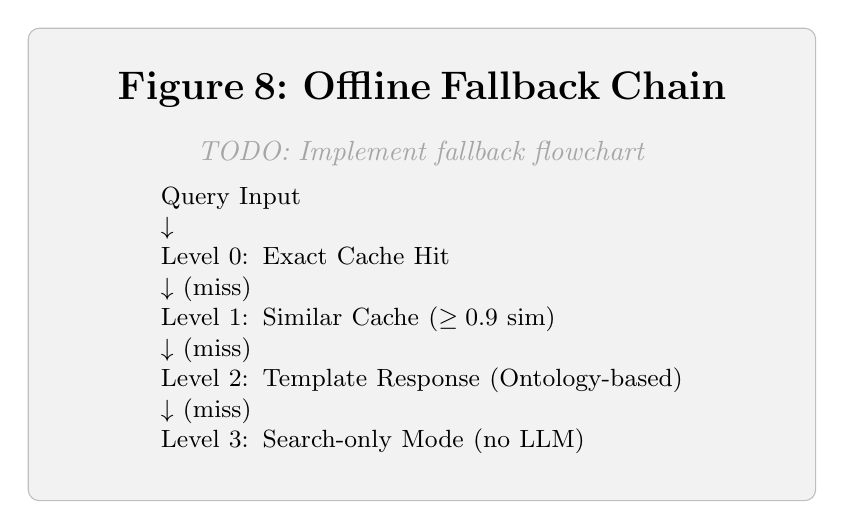
\begin{tikzpicture}
  \node[rectangle, draw=gray!50, fill=gray!10, minimum width=10cm, minimum height=6cm, rounded corners] (placeholder) {};
  \node[text width=9cm, align=center] at (placeholder.center) {
    \textbf{\Large Figure 8: Offline Fallback Chain}\\[1em]
    \textcolor{gray!70}{\textit{TODO: Implement fallback flowchart}}\\[0.5em]
    \small
    \begin{tabular}{l}
    Query Input \\
    $\downarrow$ \\
    Level 0: Exact Cache Hit \\
    $\downarrow$ (miss) \\
    Level 1: Similar Cache ($\geq 0.9$ sim) \\
    $\downarrow$ (miss) \\
    Level 2: Template Response (Ontology-based) \\
    $\downarrow$ (miss) \\
    Level 3: Search-only Mode (no LLM) \\
    \end{tabular}
  };
\end{tikzpicture}
\caption{Four-level fallback strategy enabling offline operation without LLM: exact cache lookup, similar query matching, ontology-based template responses, and search-only mode.}
\label{fig:fallback}
\end{figure}

\fbox{\parbox{0.9\textwidth}{\centering\vspace{2cm}
\textit{[Figure Placeholder: Offline Fallback Chain]}
\vspace{2cm}}}
\caption{Offline Fallback Chain. Query Processing $\rightarrow$ Exact Cache $\rightarrow$ Hybrid Retrieval $\rightarrow$ LLM Generation $\rightarrow$ (실패 시) Similar Cache $\rightarrow$ Template Response $\rightarrow$ Search Only.}
\label{fig:fallback}
\end{figure}

\cref{tab:fallback-stages}에 폴백 단계별 동작을 정리하였다.

\begin{table}[htbp]
\centering
\caption{오프라인 폴백 단계}
\label{tab:fallback-stages}
\begin{tabular}{@{}lll@{}}
\toprule
\textbf{폴백 단계} & \textbf{동작} & \textbf{언제 사용} \\
\midrule
Similar Cache & 이전 유사 질의 응답 재활용 & 반복/유사 질의 시 \\
Template Response & 온톨로지 기반 정형 응답 생성 & 간단한 조회 시 \\
Search Only & LLM 없이 검색 결과만 반환 & LLM 완전 불가 시 \\
\bottomrule
\end{tabular}
\end{table}

%------------------------------------------------------------------------------
\subsection{런타임 검증 및 신뢰도 표시}
\label{sec:method:verification}

엣지 환경에서 LLM의 환각(hallucination) 위험을 완화하기 위해, 시스템은 응답 생성 시점에 다음과 같은 런타임 검증 메커니즘을 수행한다.

\subsubsection{근거 추적 (Source Attribution)}
\label{sec:method:verification:attribution}

생성된 응답의 각 주장에 대해 근거 문서를 명시적으로 연결한다.

\textbf{구현 방식}:
\begin{enumerate}
    \item LLM 프롬프트에 검색된 문서와 함께 ``근거를 명시하라''는 지시 포함
    \item 응답 생성 후, 주장-문서 간 임베딩 유사도 계산
    \item 유사도가 임계값(0.7) 미만인 주장에 대해 경고 표시
\end{enumerate}

\subsubsection{런타임 환각 감지}
\label{sec:method:verification:hallucination}

% TODO: Figure 9 - See figures/fig-hallucination-detection.tex
\begin{figure}[htbp]
\centering
% \input{figures/fig-hallucination-detection}
\fbox{\parbox{0.9\textwidth}{\centering\vspace{2cm}
\textit{[Figure Placeholder: Runtime Hallucination Detection Pipeline]}
\vspace{2cm}}}
\caption{Runtime Hallucination Detection Pipeline. Claim Extraction $\rightarrow$ Evidence Matching $\rightarrow$ Consistency Check $\rightarrow$ 신뢰도 산출 (HIGH/MEDIUM/LOW).}
\label{fig:hallucination-detection}
\end{figure}

\subsubsection{수치 정보 검증}
\label{sec:method:verification:numeric}

농업 도메인에서 수치 정보의 정확성은 특히 중요하다. 다음과 같은 규칙 기반 검증을 적용한다 (\cref{tab:numeric-verification}).

\begin{table}[htbp]
\centering
\caption{수치 정보 검증 규칙}
\label{tab:numeric-verification}
\begin{tabular}{@{}lll@{}}
\toprule
\textbf{검증 항목} & \textbf{방법} & \textbf{예시} \\
\midrule
범위 검증 & 도메인 지식 기반 허용 범위 & 수온 10--25\textcelsius, pH 5.5--7.5 \\
일관성 검증 & 근거 문서 내 수치와 비교 & 응답 ``18\textcelsius'' vs 문서 ``18\textcelsius'' \checkmark \\
단위 검증 & 단위 변환 정확성 확인 & EC 2.5 dS/m $\neq$ 2500 $\mu$S/cm 표기 주의 \\
\bottomrule
\end{tabular}
\end{table}

\subsubsection{신뢰도 표시 및 폴백}
\label{sec:method:verification:confidence}

최종 응답에는 다음 정보가 함께 제공된다:

\begin{lstlisting}[style=jsonstyle, caption={Response Output Format}, label={lst:response-format}]
{
  "answer": "The optimal water temperature for wasabi is 13-17C...",
  "confidence": "HIGH",
  "sources": [
    {"chunk_id": "chunk_042", "title": "Wasabi Cultivation Manual",
     "page": 15, "similarity": 0.92}
  ],
  "warnings": [],
  "fallback_used": false
}
\end{lstlisting}

\cref{tab:confidence-levels}에 신뢰도 수준 정의를 정리하였다.

\begin{table}[htbp]
\centering
\caption{신뢰도 수준 정의}
\label{tab:confidence-levels}
\begin{tabular}{@{}lll@{}}
\toprule
\textbf{수준} & \textbf{조건} & \textbf{사용자 안내} \\
\midrule
HIGH & 모든 주장에 유사도 $\geq$0.8 근거 존재 & 응답 신뢰 가능 \\
MEDIUM & 일부 주장만 근거 확인 ($\geq$60\%) & 추가 확인 권장 \\
LOW & 근거 확인 불가 ($<$60\%) & 전문가 상담 권장 \\
\bottomrule
\end{tabular}
\end{table}

%------------------------------------------------------------------------------
\subsection{관련 연구와의 차별점}
\label{sec:method:comparison}

\subsubsection{EdgeRAG vs ERA-SmartFarm-RAG}
\label{sec:method:comparison:edgerag}

\cref{tab:edgerag-comparison}에 EdgeRAG~\cite{seemakhupt2024edgerag}와의 비교를 정리하였다.

\begin{table}[htbp]
\centering
\caption{EdgeRAG vs ERA-SmartFarm-RAG 비교}
\label{tab:edgerag-comparison}
\begin{tabular}{@{}lll@{}}
\toprule
\textbf{구분} & \textbf{EdgeRAG} & \textbf{ERA-SmartFarm-RAG} \\
\midrule
최적화 초점 & 범용 메모리 최적화 & 도메인 특화 + 엣지 배포 \\
인덱싱 전략 & 온라인 계층적 인덱싱 & 오프라인 사전 인덱싱 + mmap \\
검색 채널 & 단일 Dense & \textbf{Dense + Sparse + PathRAG} \\
그래프 활용 & 없음 & \textbf{인과관계 그래프} \\
도메인 지식 & 범용 & \textbf{농업 온톨로지 6개 유형} \\
메모리 절감 & 계층적 로딩 50\%$\downarrow$ & \textbf{양자화 75\%$\downarrow$ + mmap} \\
오프라인 지원 & 제한적 & \textbf{폴백 체인} \\
\bottomrule
\end{tabular}
\end{table}

\subsubsection{MobileRAG 패턴 비교}
\label{sec:method:comparison:mobilerag}

\begin{table}[htbp]
\centering
\caption{MobileRAG 패턴 비교}
\label{tab:mobilerag-comparison}
\begin{tabular}{@{}lll@{}}
\toprule
\textbf{구분} & \textbf{MobileRAG (EcoVector+SCR)} & \textbf{ERA-SmartFarm-RAG} \\
\midrule
인덱스 파티셔닝 & k-means 클러스터 계층 & FAISS mmap (전체 인덱스) \\
부분 로딩 & 클러스터별 on-demand & mmap lazy load (OS 페이지 캐시) \\
토큰 절감 & SCR (Selective Content Reduction) & \textbf{Semantic Dedup + Crop Filter} \\
런타임 & AI Edge / MLX & \textbf{llama.cpp GGUF} \\
\bottomrule
\end{tabular}
\end{table}

\subsubsection{핵심 차별점}
\label{sec:method:comparison:summary}

\begin{enumerate}
    \item \textbf{도메인 특화}: 범용 메모리 최적화 대신 농업 온톨로지와 인과관계 그래프 활용
    \item \textbf{3채널 검색}: 수치/단위 정보(EC, pH)의 정확한 매칭을 위한 Sparse 채널 유지
    \item \textbf{경량 Context Shaping}: SCR 대신 Semantic Dedup + Crop Filter (구현 단순화)
    \item \textbf{완전 오프라인}: Template Responder로 LLM 없이도 기본 응답 가능
\end{enumerate}

% ==============================================================================
% END OF METHODOLOGY SECTION
% ==============================================================================
